\chapter{Discussion} \label{ch:discussion}

\section{Threshold calibration}
Different localization methods exhibit different localization performance distributions, as illustrated in Fig. \ref{fig:boxacc_resnet50_imagenet}. Here we show the box accuracy (BoxAccV2 as defined in equation \ref{eq:boxaccv2}) using different localization methods for the ResNet-50 network on the ImageNet validation dataset. We use a BoxAcc plot to illustrate box accuracy in function of the score map threshold. Fig. \ref{fig:boxacc_resnet50_imagenet} clearly shows that each localization method has a different BoxAcc distribution. Fixing the score map threshold at a single pre-defined value, could lead to increased performance of some methods and to decreased performance for others. 

The threshold-independent localization metric MaxBoxAccV3 recall (MaxBoxAccV3 in short) is then the maximum value of the BoxAcc metric in the plot. The optimal score map threshold is the score map threshold for the maximum box accuracy. We observe that the localization methods have different optimal score map thresholds, but the MaxBoxAccV3 values are not significantly different. This provides an explanation of the limited differences between localization methods for MaxBoxAccV3 recall as observed in Table \ref{tab:metrics_resnet50_imagenet}.

\begin{figure}[ht]
    \begin{center}       
    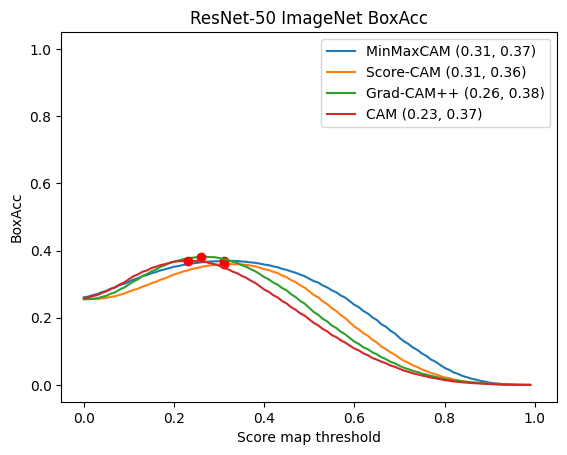
\includegraphics[width=0.7\textwidth]{fig_boxacc_resnet50_imagenet.png}
    \caption[BoxAcc (IoU 50)for ResNet-50 on ImageNet]{Performance at varying operating thresholds. BoxAcc($\tau$) versus score map threshold $\tau$ at IoU threshold 50 for ResNet-50 on ImageNet.}
    \caption*{Source: Author}
    \label{fig:boxacc_resnet50_imagenet}
    \end{center}
\end{figure}

\section{Classification versus localization accuracy}
When comparing classification accuracy with localization accuracy (MaxBoxAccV3 recall) during training, we observed that there is a correlation between both metrics. Fig. \ref{fig:loc_vs_acc_vgg16_gap_cam_synthetic} illustrates that classification accuracy and CAM localization accuracy (MaxBoxAccV3 recall) for VGG16-GAP on each of the validation synthetic datasets, improve during the early epochs of training, until both metrics start converging.

In some cases, the best localization performances are achieved before convergence. At early epochs, the localization can fluctuate a lot and thus, peak performance could be noise, rather than real performance. Fig. \ref{fig:loc_vs_acc_resnet50_cam_d1b} illustrates this for the CAM localization method on ResNet-50 for the d1b synthetic dataset. To avoid measuring noise, we use an early stop criterion that stops training when classification accuracy has not improved the best accuracy during 5 epochs. We take as localization accuracy the value computed at the last epoch on the validation dataset.

\begin{figure}[ht]
\begin{center}
    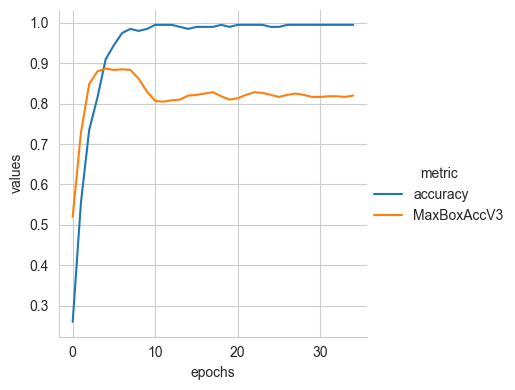
\includegraphics[width=0.4\textwidth]{images/fig_loc_vs_acc_resnet50_cam_d1b.png}
    \caption[Classification versus CAM localization accuracy on VGG16-GAP for d1b dataset]{Classification versus CAM localization accuracy on VGG16-GAP for d1b dataset.}
    \caption*{Source: Author}
    \label{fig:loc_vs_acc_resnet50_cam_d1b}
\end{center}
\end{figure}

% The second example is shown in Fig. \ref{fig:loc_vs_acc_vgg16_gap_minmaxcam_synthetic}.

Rework:
% We illustrate this in Fig. \ref{fig:classification_versus_localization} for the MinMaxCAM method where we show the training curves of the classification accuracy and localization accuracy on the synthetic validation dataset for the ResNet-50 network. 

%During the early training epochs, both classification accuracy and localization accuracy improve. But in further epochs, classification accuracy keeps improving, while localization performance drops until they both converge.

%The result shows that localization and classification performance may not necessarily correlate and further classification training may hurt localization performance. As classification accuracy improves, the model focuses on learning the most discriminative parts of an object to classify the image correctly. These discriminative parts only partially cover an object. As the localization objective is to cover the full object region, improving classification performance decreases localization accuracy. 

%Therefore, it's important to use localization-only metrics like MaxBoxAccV3 and PxAP for model selection and evaluation of WSOL methods. To avoid learning a model which focuses on optimizing classification performance only, we stop the learning process when the validation loss hasn't decreased for five consecutive epochs.
